\documentclass[17pt]{extarticle}
\usepackage{amsmath, amssymb}
\usepackage{nccmath}
\usepackage[a4paper, total={6.5in, 9in},top=2mm,left=27mm]{geometry}
\usepackage{titlesec}
\usepackage{tikz}


%\titleformat*{\section}{\fontsize{17}{20}\selectfont}


\titleformat{\section}
{\normalfont\normalsize\bfseries}{\thesection}{1em}{}

\setcounter{secnumdepth}{0} %% no numbering for sections

\begin{document}
\noindent
\begin{fleqn} 

%----------------------------------------

\section{Question: 01}
A box is made with a square base and open top. The area of material for making the box is 300 sq. cm. Find the dimensions of the box, if its volume is maximum. Also find the maximum volume.

%----------------------------------------


\section{Answer: 01}


Let  'x'  be the side of a square base and  'h' be the height of the box.\\
$\therefore$ Total surface area = $x^2+4h = 300\,cm^2$
\[\therefore h = \frac{300 - x^2}{4x}\]
\begin{equation} \nonumber
\begin{alignedat}{4}
\hspace{0em}&\hspace{-0em}\text{Base Volume V}\\
&= \text{Area of Base x Height}\\
&= x^2\left(\frac{300-x^2}{4x}\right)\\
&= \frac{1}{4}(300x - x^2)
\end{alignedat}
%\vrule
\quad\quad\quad
\begin{alignedat}{4}
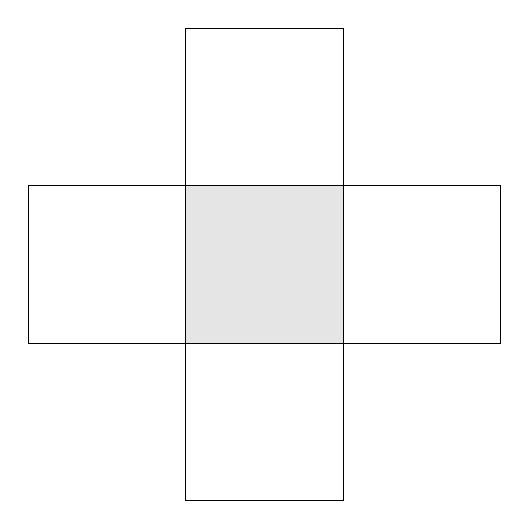
\begin{tikzpicture}
\draw (0,0) -- (0,2) -- (2,2) -- (2,4) -- (4,4) -- (4,2) -- (6,2) -- (6,0) -- (4,0) -- (4,-2) -- (2,-2) -- (2,0) -- (0,0) ; 
\filldraw[fill=gray!20] (2,0) rectangle (4,2);
\end{tikzpicture}
\end{alignedat}
\end{equation}
\quad


\begin{equation} \nonumber
\begin{alignedat}{4}
& \frac{dV}{dx}=\frac{1}{4}(300x - x^2) \\
& But\  \frac{dV}{dx}= 0 \text{ for max}\\
& \therefore \frac{1}{4}(300x - x^2)=0\\
& \therefore x = \pm 10\\
& \therefore x = 10 \ \ (+ve)
\end{alignedat}
\quad
\vrule
\quad
\begin{alignedat}{4}
&= \left(\frac{d^2V}{dx^2}\right)_{x=10}=\left(\frac{-3x}{2}\right)_{x=10} = -15<0\\
& \therefore \text{ V is max at x = 10 by 2nd derivative test}\\
& \therefore Height\  h=But\  \frac{300 - (10)^2}{4(10)}= 5\ cm\\
& \therefore Required\  dim = 5 \times  5 \times 10 \\
& Consequently \ Volume\ V = 500 \ cm^3 \\
\end{alignedat}
\end{equation}
%----------------------------------------

\section{Question: 02}

\begin{equation} \nonumber
\begin{alignedat}{4}
& Evlauate :\ \  \int \frac{x^5 - 4x^3 + 6x}{x}\ dx\\
\end{alignedat}
\end{equation}


%----------------------------------------

\section{Answer: 02}

\begin{equation} \nonumber
\begin{alignedat}{4}
& \quad \int \frac{x^5 - 4x^3 + 6x}{x}\ dx\\
&= \int x^4 - 4x^2 +6)dx\\
\end{alignedat}
\quad
\vrule
\quad
\begin{alignedat}{4}
\begin{tikzpicture}
\draw (0,0) rectangle (3,3);
\end{tikzpicture}
\end{alignedat}
\end{equation}
\quad
%----------------------------------------


\end{fleqn}
\end{document} 